\documentclass[a4paper,twoside]{article}

\usepackage{epsfig}
\usepackage{subfigure}
\usepackage{calc}
\usepackage{amssymb}
\usepackage{amstext}
\usepackage{amsmath}
\usepackage{amsthm}
\usepackage{multicol}
\usepackage{pslatex}
\usepackage{apalike}
\usepackage{SCITEPRESS}     % Please add other packages that you may need BEFORE the SCITEPRESS.sty package.

\subfigtopskip=0pt
\subfigcapskip=0pt
\subfigbottomskip=0pt

\begin{document}

\title{Authors' Instructions  \subtitle{Preparation of Camera-Ready Contributions to SCITEPRESS Proceedings} }

\author{\authorname{First Author Name\sup{1}, Second Author Name\sup{1} and Third Author Name\sup{2}}
\affiliation{\sup{1}Institute of Problem Solving, XYZ University, My Street, MyTown, MyCountry}
\affiliation{\sup{2}Department of Computing, Main University, MySecondTown, MyCountry}
\email{\{f\_author, s\_author\}@ips.xyz.edu, t\_author@dc.mu.edu}
}

\keywords{The paper must have at least one keyword. The text must be set to 9-point font size and without the use of bold or italic font style. For more than one keyword, please use a comma as a separator. Keywords must be titlecased.}

\abstract{The abstract should summarize the contents of the paper and should contain at least 70 and at most 200 words. The text must be set to 9-point font size.}

\onecolumn \maketitle \normalsize \vfill

\section{\uppercase{Introduction}}
\label{sec:introduction}

\noindent Your paper will be part of the conference proceedings
therefore we ask that authors follow the guidelines explained in
this example in order to achieve the highest quality possible
\cite{Smith98}.

Be advised that papers in a technically unsuitable form will be
returned for retyping. After returned the manuscript must be
appropriately modified.

\section{\uppercase{Manuscript Preparation}}

\noindent We strongly encourage authors to use this document for the
preparation of the camera-ready. Please follow the instructions
closely in order to make the volume look as uniform as possible
\cite{Moore99}.

Please remember that all the papers must be in English and without
orthographic errors.

Do not add any text to the headers (do not set running heads) and
footers, not even page numbers, because text will be added
electronically.

For a best viewing experience the used font must be Times New
Roman, except on special occasions, such as program code
\ref{subsubsec:program_code}.


\subsection{Manuscript Setup}

\noindent The template is composed by a set of 7 files, in the
following 2 groups:\\
\noindent {\bf Group 1.} To format your paper you will need to copy
into your working directory, but NOT edit, the following 4 files:
\begin{verbatim}
  - apalike.bst
  - apalike.sty
  - article.cls
  - scitepress.sty
\end{verbatim}

\noindent {\bf Group 2.} Additionally, you may wish to copy and edit
the following 3 example files:
\begin{verbatim}
  - example.bib
  - example.tex
  - scitepress.eps
\end{verbatim}


\subsection{Page Setup}

The paper size must be set to A4 (210x297 mm). The document
margins must be the following:

\begin{itemize}
    \item Top: 3,3 cm;
    \item Bottom: 4,2 cm;
    \item Left: 2,6 cm;
    \item Right: 2,6 cm.
\end{itemize}

It is advisable to keep all the given values because any text or
material outside the aforementioned margins will not be printed.

\subsection{First Section}

This section must be in one column.

\vfill
\subsubsection{Title and Subtitle}

Use the command \textit{$\backslash$title} and follow the given structure in "example.tex". The title and subtitle must be with initial letters
capitalized (titlecased). If no subtitle is required, please remove the corresponding \textit{$\backslash$subtitle} command. In the title or subtitle, words like "is", "or", "then", etc. should not be capitalized unless they are the first word of the subtitle. No formulas or special characters of any form or language are allowed in the title or subtitle.

\subsubsection{Authors and Affiliations}

Use the command \textit{$\backslash$author} and follow the given structure in "example.tex".

\subsubsection{Keywords}

Use the command \textit{$\backslash$keywords} and follow the given structure in "example.tex". Each paper must have at least one keyword. If more than one is specified, please use a comma as a separator. The sentence must end with a period.

%\subsubsection{Abstract}
%Use the command \textit{$\backslash$abstract} and follow the given structure in "example.tex".
%Each paper must have an abstract up to 200 words. The sentence must end with a period.


\vfill

%\subsubsection{Subsection Titles.. \& Sub-Subsection Titles}
%The heading of a subsection title must be with initial letters
%capitalized (titlecased).
%Words like "is", "or", "then", etc. should not be capitalized unless
%they are the first word of the subsection title.
%Example: \textit{$\backslash$subsection\{First Subtitle\}}

%Example: \textit{$\backslash$begin\{figure*\}}
%\hspace*{1.5cm}\textit{$\backslash$end\{figure*\}}

% Figures should be centered and should always have a caption
% positioned under it. The font size to use is 9-point. No bold or
% italic font style should be used.

% {
\epsfig{file = SCITEPRESS.eps, width = 5.5cm}}

\subsection{Anonymization}

\begin{figure*}[!h]
	%\vspace{-0.2cm}
	\centering
	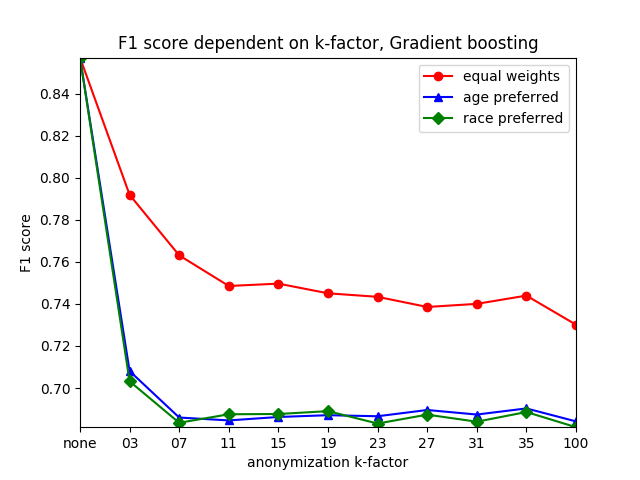
\includegraphics[width=0.49\textwidth]{figures/anonymization/adults_marital_status/gradient_boost}
	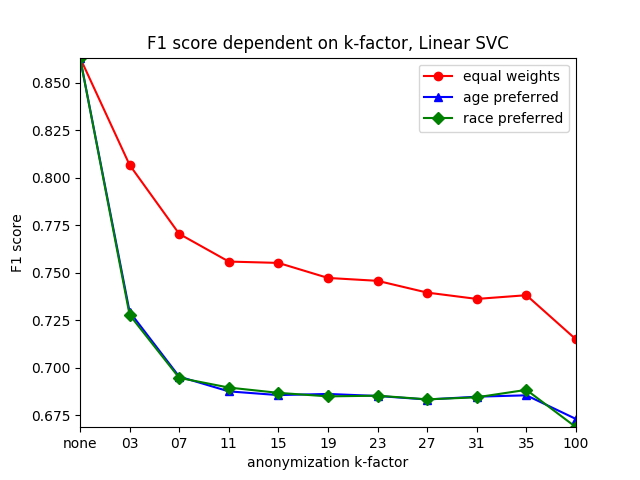
\includegraphics[width=0.49\textwidth]{figures/anonymization/adults_marital_status/linear_svc}
	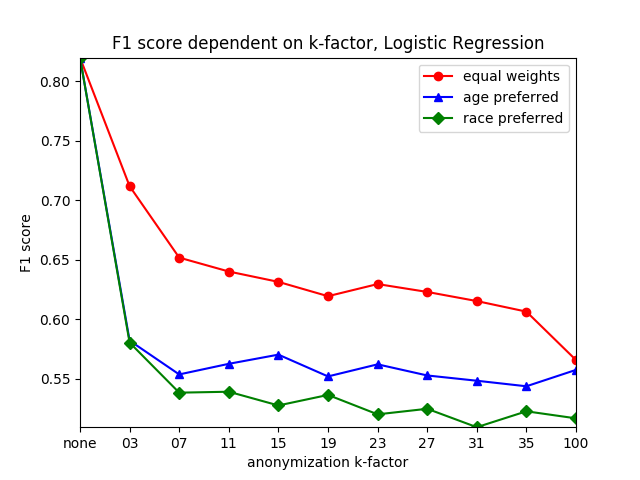
\includegraphics[width=0.49\textwidth]{figures/anonymization/adults_marital_status/logistic_regression}
	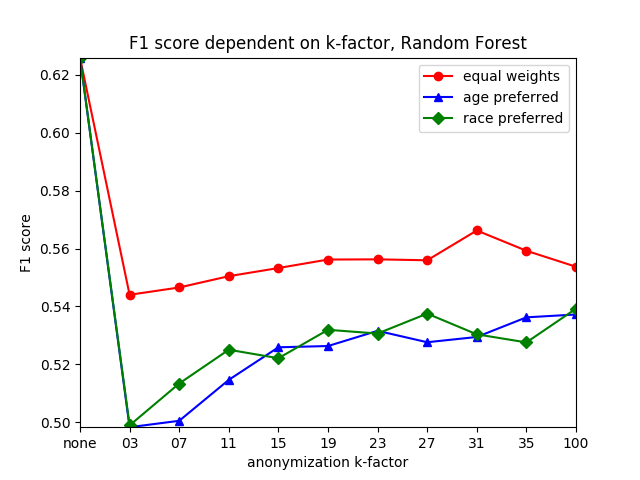
\includegraphics[width=0.49\textwidth]{figures/anonymization/adults_education_num/random_forest}
	\caption{This caption has one line so it is centered.}
	\label{fig:results_anonymization_marital_status}
\end{figure*}

\begin{figure*}[!h]
	%\vspace{-0.2cm}
	\centering
	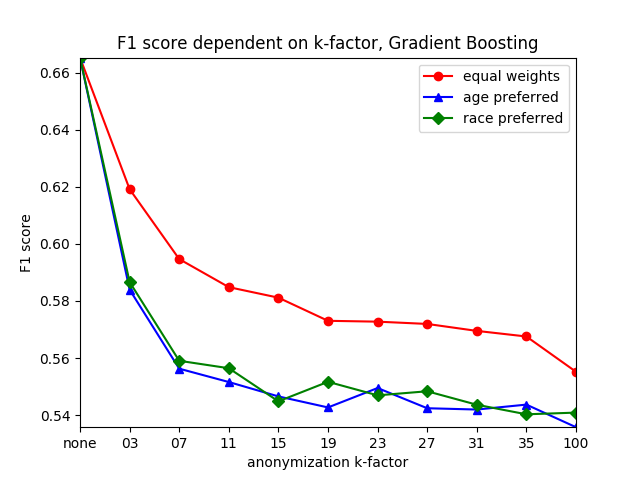
\includegraphics[width=0.49\textwidth]{figures/anonymization/adults_education_num/gradient_boost}
	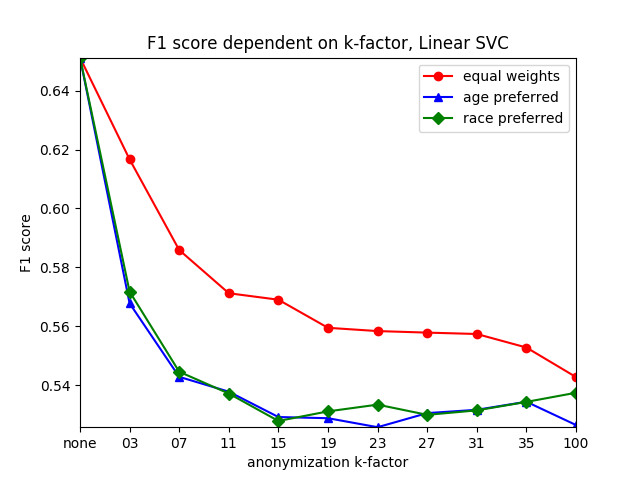
\includegraphics[width=0.49\textwidth]{figures/anonymization/adults_education_num/linear_svc}
	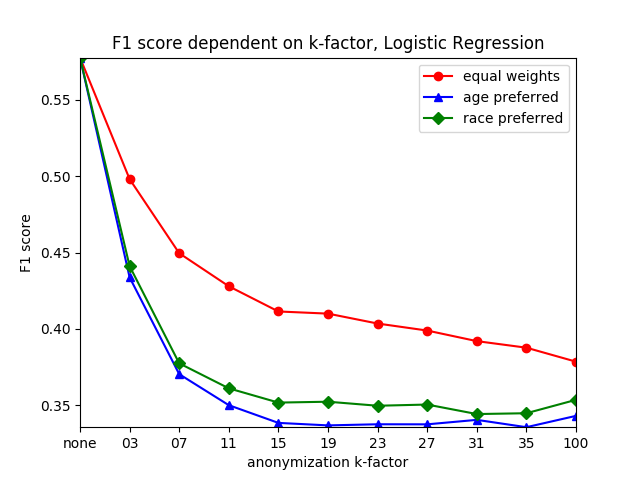
\includegraphics[width=0.49\textwidth]{figures/anonymization/adults_education_num/logistic_regression_lbfgs}
	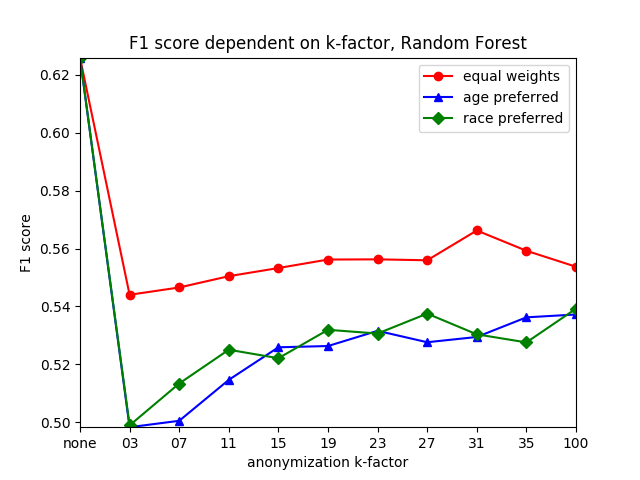
\includegraphics[width=0.49\textwidth]{figures/anonymization/adults_education_num/random_forest}
	\caption{This caption has one line so it is centered.}
	\label{fig:results_anonymization_education_num}
\end{figure*}


\subsection{Perturbation}

\begin{figure*}[h]
	%\vspace{-0.2cm}
	\centering
	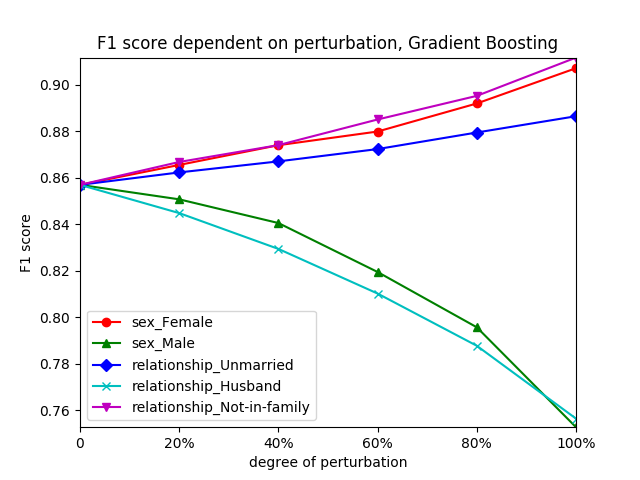
\includegraphics[width=0.49\textwidth]{figures/perturbation/adults_marital_status/gradient_boost}
	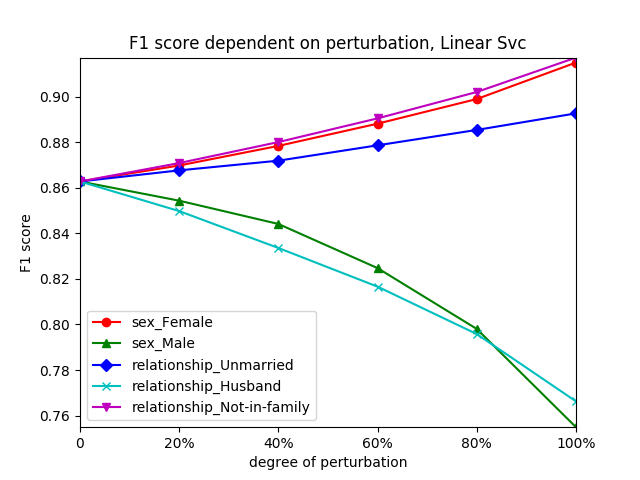
\includegraphics[width=0.49\textwidth]{figures/perturbation/adults_marital_status/linear_svc}
	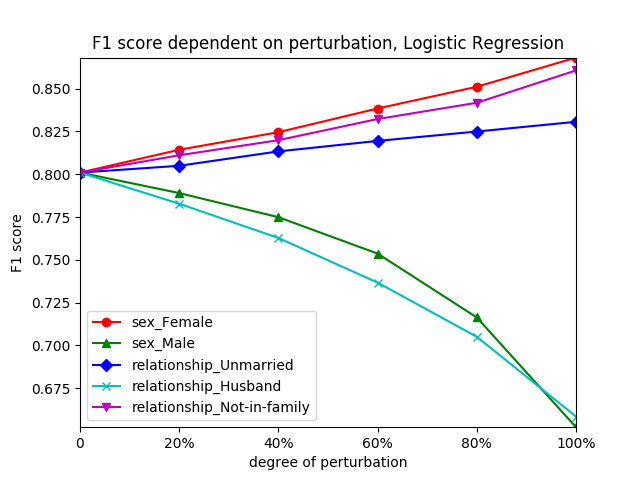
\includegraphics[width=0.49\textwidth]{figures/perturbation/adults_marital_status/logistic_regression}
	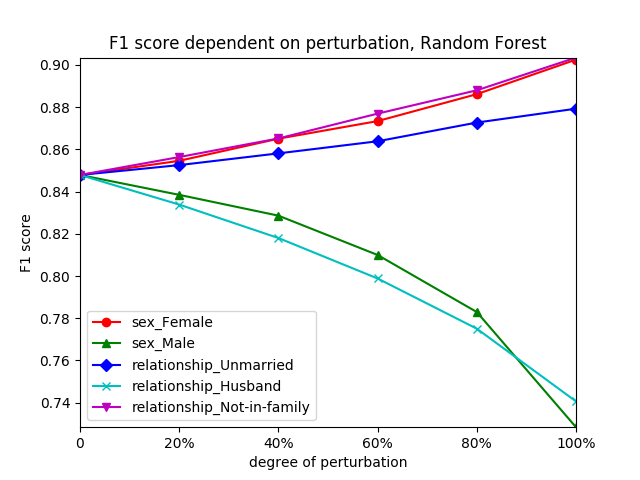
\includegraphics[width=0.49\textwidth]{figures/perturbation/adults_marital_status/random_forest}
	\caption{This caption has one line so it is centered.}
	\label{fig:results_anonymization_education_num}
\end{figure*}

We expected a steady decline in the quality of classification results over all three scenarios: 1) anonymization of datasets, 2) perturbation by selectively deleting attribute values of positive significance w.r.t the result, 3) perturbation by selectively deleting attribute values of negative significance w.r.t the result.

The actual results satisfied our expectations only in the first two cases, with the shape of the actual outcomes being a little bit surprising. As can be seen in Figure~\ref{fig:adult_results_anonymization}, the F1 score of all algorithms applied declines more drastically at the beginning, with more benign further losses as the $k$-factor of anonymization increases. Whereas the F1 curves for gradient boosting, linear SVC and logistic regression approximate a $1/x$ curve, the random forest classifier reacts more sensitively to even slight anonymization, but seems to stay more robust with higher values of $k$.

Considering the exact performance, Linear SVC and logistic regression yielded the worst outcomes under anonymization, which is not further surprising given their lower scores on the original input data to begin with.

\begin{figure*}[h]
	%\vspace{-0.2cm}
	\centering
	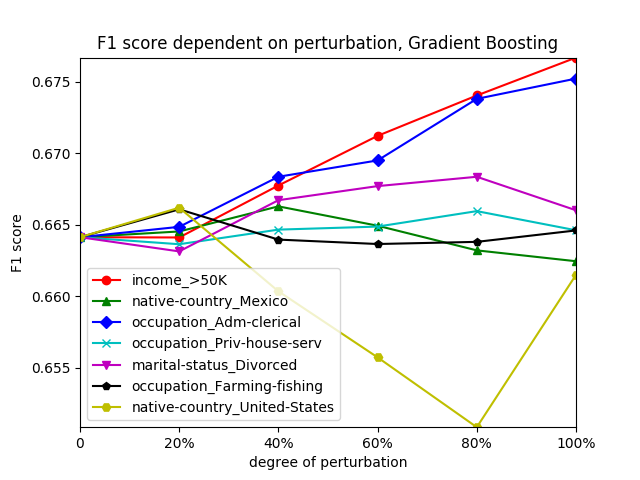
\includegraphics[width=0.49\textwidth]{figures/perturbation/adults_education_num/gradient_boost}
	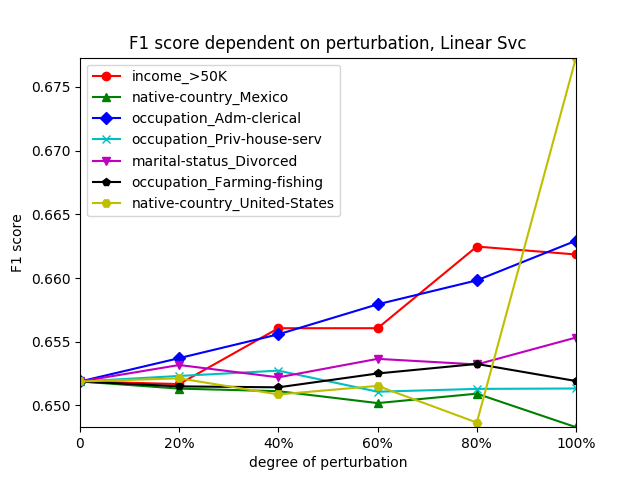
\includegraphics[width=0.49\textwidth]{figures/perturbation/adults_education_num/linear_svc}
	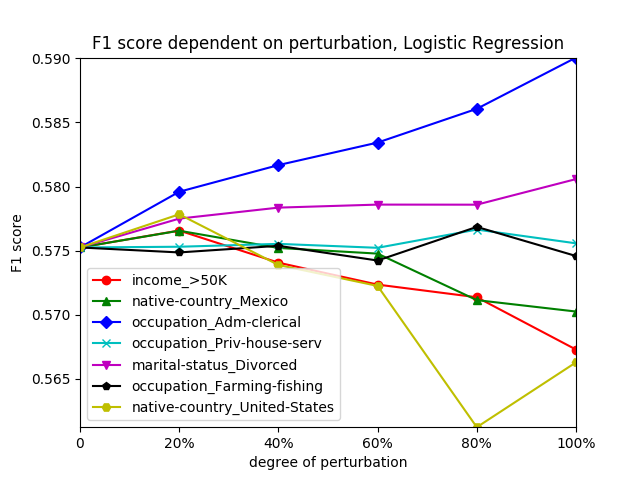
\includegraphics[width=0.49\textwidth]{figures/perturbation/adults_education_num/logistic_regression}
	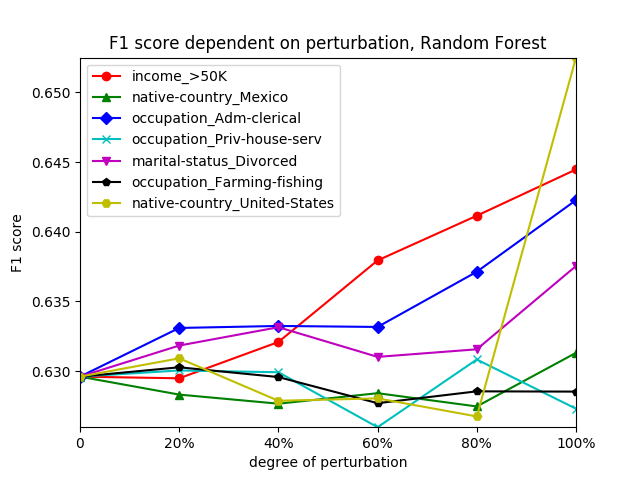
\includegraphics[width=0.49\textwidth]{figures/perturbation/adults_education_num/random_forest}
	\caption{This caption has one line so it is centered.}
	\label{fig:results_anonymization_education_num}
\end{figure*}






\begin{equation}\label{eq1}
    a=b+c
\end{equation}

\subsubsection{Program Code}\label{subsubsec:program_code}


\begin{small}
\begin{verbatim}
 Begin
     Writeln('Hello World!!');
 End.
\end{verbatim}
\end{small}


\cite{DuchiJordan:2014:PrivacyAwareLearning}
\cite{iMLExperiment}


\section{\uppercase{Conclusions}}
\label{sec:conclusion}

\noindent In this paper we presented...

%\section*{\uppercase{Acknowledgements}}

%\noindent If any, should be placed before the references section
%without numbering. To do so please use the following command:
%\textit{$\backslash$section*\{ACKNOWLEDGEMENTS\}}


\vfill
\bibliographystyle{apalike}
{\small
\bibliography{references}}


%\section*{\uppercase{Appendix}}

%\noindent If any, the appendix should appear directly after the
%references without numbering, and not on a new page. To do so please use the following command:
%\textit{$\backslash$section*\{APPENDIX\}}

\vfill
\end{document}

